\documentclass[stu, 12pt, letterpaper, donotrepeattitle, floatsintext, natbib]{apa7}
\usepackage[utf8]{inputenc}
%\usepackage{fontspec} %paquete para usar la fuente Arial 12
%\usepackage{comment}
\usepackage{marvosym}
\usepackage{graphicx}
\usepackage{float}
\usepackage{amsmath}
\usepackage[normalem]{ulem}
\usepackage[spanish]{babel}
\usepackage{lastpage} %para le formato que quiere la profe QUITAR SI QUIERES OG APA7
\usepackage{ragged2e} %para le formato que quiere la profe QUITAR SI QUIERES OG APA7
\usepackage{indentfirst} %para le formato que quiere la profe QUITAR SI QUIERES OG APA7

%comando para ajustar la fuente Arial en todo el documento
%\setmainfont{Arial} %COMPILAR DOC CON XeLateX DOS VECES

%\DeclareCaptionLabelSeparator*{spaced}{\\[2ex]}
%\captionsetup[table]{textfont=it,format=plain,justification=justified,
%  singlelinecheck=false,labelsep=spaced,skip=1pt}


\selectlanguage{spanish}

\useunder{\uline}{\ul}{}
\newcommand{\myparagraph}[1]{\paragraph{#1}\mbox{}\\}

%\rfoot{Página \thepage \hspace{1pt} de \pageref{LastPage}}%QUITAR SI QUIERES OG APA7 
\rhead{} %QUITAR SI QUIERES OG APA7
\setcounter{secnumdepth}{3} %permite enumerar las secciones QUITAR SI QUIERES OG APA7
\setlength{\parindent}{1.27cm} %sangria forzada QUITAR SI QUIERES OG APA7

\renewcommand\labelitemi{\(\bullet\)}

\newcommand*\chem[1]{\ensuremath{\mathrm{#1}}}

\begin{document}
    %PORTADA
    \begin{titlepage}
        \begin{figure}[ht]
            \centering
            
\includegraphics[width=15cm]{logosITT.png}
        \end{figure}
        \centering
        {\Large Tecnológico Nacional de México\\Instituto Tecnológico de Tijuana\par}
        \vspace{1cm}
        {\Large SCD-1015SC6C Lenguajes y Automatas I\par}
        \vspace{1cm}
        {\Large Unidad 2\par}
        \vspace{1.5cm}
        {\Large\bfseries Práctica 1\par}
        \vspace{2cm}
        {\large Lic. Gloria Leticia Morales Rios\par}
        \vfill
            {\large Abraham Jhared Flores Azcona, 19211640\par}
        \vfill
        {\large 25 de marzo de 2022}
    \end{titlepage}

% Índices
\pagenumbering{arabic}
    % Contenido
\renewcommand\contentsname{Contenido}
\tableofcontents

% Cuerpo 
    %NOTA: PARA CITAR ESTILO "Merts (2003)" usar \cite{<nombre_cita_bib>}
    %                        "(Metz, 1978)" usar \citep{<nombre_cita_bib>}
\newpage
\section{Introducción}
Muchos \begin{justifying}
    de los temas de la materia requieren especial detalle para poder ser aplicados, como los son los autómatas.
    En esta breve redacción se presentan a grandes rasgos los conceptos ligados a los autómatas y cómo se relacionan
    con las expresiones regulares.\par
    \end{justifying}
\vspace{\baselineskip}
\section{Autómatas Finitos}
\subsection{Definición formal}
Es \begin{justifying}
    una quintupla denominada \(A\): \par
\end{justifying}
\[A=\left(Q,\, V,\, \delta,\, q_0,\, F \right)\]
\begin{justifying}
    donde:
    \begin{itemize}
        \item \(Q\): Conjunto finito de estados.
        \item \(V\): Vocabulario (alfabeto) de entrada.
        \item \(\delta\): Función de transición \(\delta: Q\times V \rightarrow Q\). Generalmente se representa con una tabla.
        \item \(q_0\): Estado inicial.
        \item \(F\): Conjunto de estados finales donde \(F\neq 0, F\subset Q\).
    \end{itemize}\par
\end{justifying}
\begin{justifying}
    También se puede representar por medio de un grafo dirigido donde las flechas con etiquetas representan
    los carácteres de entrada a la máquina y los nodos con nombre representan los estados. Si un nodo tiene otro círculo,
    se interpreta que el estado que representa es un estado final. Esto nos permite comprobar si una cadena dada es aceptada
    por el lenguaje que el autómata representa.\par
\end{justifying}
\begin{figure}[H]
    \centering
    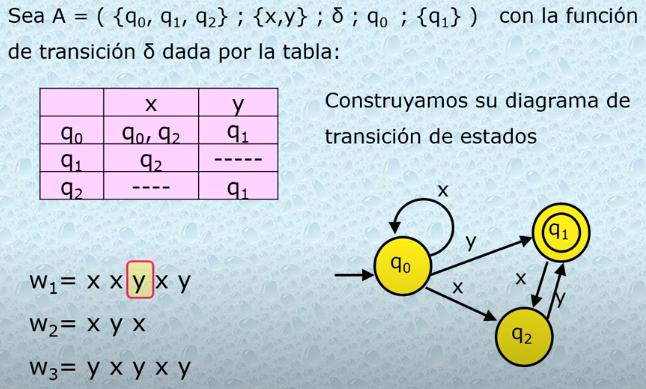
\includegraphics[width=15cm]{ejemplo_automata.png}
\end{figure}
\vspace{\baselineskip}
\subsection{Clasificación de tipos de lenguajes y máquinas que lo reconocen}
Existen \begin{justifying}
    cuatro tipos donde cada uno se reconoce por una máquina. Se dice que un lenguaje es de tipo \(k\) si y sólo si existe una gramática de
    tipo \(k\) que lo genere.\par
 \end{justifying}
 \begin{table}[]
    \centering
    \begin{tabular}{cc}
    \hline
    \textbf{Tipo} & \textbf{Máquina que los reconoce} \\ \hline
    0             & Máquina de Turing                 \\
    1             & Autómata linealmente acotado      \\
    2             & Autómata de pila                  \\
    3             & Autómata finito                   \\ \hline         
    \end{tabular}
    \end{table}
\subsection{Clasificación de los Automatas Finitos}
Tenemos \begin{justifying}
    dos clasificaciones: \emph{No determinísticos y determinísticos}.\par
\end{justifying}
\begin{justifying}
    \begin{itemize}
        \item \emph{No determinísticos:} si no cumplen las condiciones para ser determinísticos.
        \item \emph{Determinísticos:} no tiene transiciones por medio de \(\lambda\) y \(\delta\) cumple con la propiedad de unicidad, que quiere decir que \(\delta\) solo cambia a un solo estado.
    \end{itemize}\par    
\end{justifying}
\subsection{Reglas del metodo para obtener una expresión regular a partir de un automata finito}
Se \begin{justifying}
    tienen 5 reglas:
    \begin{enumerate}
        \item Si \(\delta(p, a)=q\) entonces \(p=aq\).
        \item Si \(\delta(p, a)=q\) y \(\delta(p, b)=r\) entonces \(p=aq+br\).
        \item Si \(\delta(p, a)=p\) entonces \(p=a^*\).
        \item Si \(\delta(p, a)=p\) y \(\delta(p, b)=r\) entonces \(p=ap+bq=a^*\cdot (bq)\).
        \item Si \(p\in F\) entonces \(p=\lambda\).
    \end{enumerate}\par
\end{justifying}
\vspace{\baselineskip}
\subsection{Construcción de un autómata finito dado un lenguaje}
Se \begin{justifying}
    utiliza el siguiente ejemplo para entender de mejor manera el proceso. A grandes rasgos se da la expresión formal
y se debe de descifrar el grafo de la maquina a partir del formalismo. A continuación se muestra un ejemplo de ello.\par
\end{justifying}
\subsubsection{Ejemplo}
Construye \begin{justifying}
    el autómata finito dado el siguiente lenguaje:\par
\end{justifying}
\[L=\{(ab)^mca^p\,|\,w \text{ comienza con }a\land w \text{ no contiene la secuencia }bc\}\]
\begin{figure}[H]
    \centering
    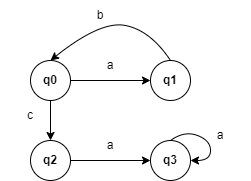
\includegraphics[width=7cm, height=4cm]{ejemplo_construct.png}
\end{figure}
\vspace{\baselineskip}
\subsection{Ejercicios}
\subsubsection{Indicar si los siguientes autómatas son determinístas}
\begin{figure}[H]
    \centering
    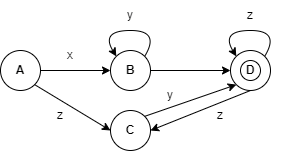
\includegraphics[width=7cm, height=4cm]{automata1_ej1.png}
\end{figure}
Debido \begin{justifying}
    a que \(\delta(D,z)=(C, D)\), \(\#(C, D)=2\) que rompe el principio de unicidad, que
    nos dice que \(\#\delta(q,a)=1\) implica que éste autómata no es determinista.\par
\end{justifying}
\begin{figure}[H]
    \centering
    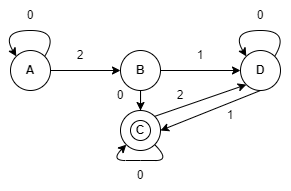
\includegraphics[width=7cm, height=4cm]{automata2_ej1.png}
\end{figure}
Debido \begin{justifying}
    a que todos las transiciones cumplen que \(\#\delta(q,a)=1\), el autómata dado es determinista.\par
\end{justifying}
\begin{figure}[H]
    \centering
    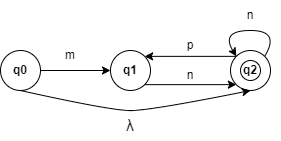
\includegraphics[width=7cm, height=4cm]{automata3_ej1.png}
\end{figure}
Debido \begin{justifying}
    a que una transición se realiza con \(\lambda\), implica que el autómata no es determinista.\par
\end{justifying}
\vspace{\baselineskip}
\subsubsection{Indicar cual de estas E.R. corresponde al lenguaje que reconoce segun la tabla \(\delta\)}
\begin{enumerate}
    \item \(1^*0(10^*1\lor 0^*)^*\)
    \item \(1^*00^*(10^*1)^*\)
\end{enumerate}
\begin{table}[]
    \centering
    \begin{tabular}{c|cc}
    \cline{2-3}
    \multicolumn{1}{l|}{} & \textbf{0} & \textbf{1} \\ \hline
    \textbf{a}            & b          & a          \\
    \textbf{b}            & b          & c          \\
    \textbf{c}            & c          & b          \\ \hline
    \end{tabular}
    \end{table}
\begin{figure}[H]
    \centering
    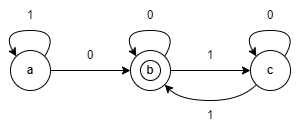
\includegraphics[width=7cm, height=4cm]{automata_ej2.png}
\end{figure}
\vspace{\baselineskip}
La \begin{justifying}
    solución para esto se obtiene mediante el uso de las propiedades listadas anteriormente. Por lo que procedemos a hacerlo:
    \begin{itemize}
        \item \(\delta(a,1)=a\rightarrow 1^*\).
        \item \(\delta(a,0)=b\rightarrow 0\).
        \item \(\delta(b,1)=c\rightarrow 1\).
        \item \(\delta(b,0)=b\rightarrow 0^*\).
        \item \(b\in F\rightarrow 0^*\).
        \item \(\delta(c,0)=c\rightarrow 0^*\).
        \item \(\delta(c,1)=b\rightarrow 1\).
    \end{itemize}\par
\end{justifying}
Finalmente \begin{justifying}
    concatenamos las expresiones. Notese que existen bucles en el estado final \(b\), las posibles expresiones pueden ser 
\(10^*1\) ó solamente \(0^*\) por lo que la expresión regular resultante es \(1^*0(10^*1\lor 0^*)^*\), indicando que 1) es la
expresión regular que se reconoce en el autómata.\par
\end{justifying}
\vspace{\baselineskip}
\section{Conclusión}
Las \begin{justifying}
    mecanicas de los autómatas nos permiten comprender la complejidad del análisis que se debe hacer previo al desarrollo
    de un lenguaje de programación. Aparte de que ilustran los patrones que se pueden hacer dado ese lenguaje.\par
    \end{justifying}
\end{document}